% =====================================================================
% What two etch-rate measurements constrain:
% identifiability and EEDF sensitivity of a reduced SF6 ICP model
%
% Path A consolidated manuscript.
% Build with:  pdflatex manuscript && bibtex manuscript && pdflatex manuscript && pdflatex manuscript
% =====================================================================
\documentclass[11pt,a4paper]{article}

\usepackage[margin=1in]{geometry}
\usepackage[utf8]{inputenc}
\usepackage[T1]{fontenc}
\usepackage{amsmath,amssymb,amsthm}
\usepackage{graphicx}
\usepackage{booktabs}
\usepackage{natbib}
\usepackage{hyperref}
\usepackage{tikz}
\usetikzlibrary{arrows.meta,positioning,shapes.geometric,fit}

\hypersetup{
  colorlinks=true,
  linkcolor=blue!50!black,
  citecolor=blue!50!black,
  urlcolor=blue!60!black,
}

% --- macros ---
\newcommand{\sfsix}{SF$_6$}
\newcommand{\vth}{\bar v_{\mathrm{th}}}
\newcommand{\kdiss}{k_{\mathrm{diss}}}
\newcommand{\kiz}{k_{\mathrm{iz}}}
\newcommand{\katt}{k_{\mathrm{att}}}
\newcommand{\nel}{n_e}
\newcommand{\nSFsix}{n_{\mathrm{SF}_6,0}}

\title{What two etch-rate measurements constrain:\\
       identifiability and EEDF sensitivity of a reduced \sfsix{}
       ICP model}

\author{Zachariah Ngan\thanks{%
  Correspondence: \texttt{zngan@illinois.edu}}\\[2pt]
  \normalsize\itshape Illinois Plasma Institute}
\date{\today}

\begin{document}
\maketitle

\begin{abstract}
Reduced-order models of inductively coupled plasma (ICP) etching
reactors rely on calibrated parameters that are routinely interpreted
as physical quantities. Using a one-parameter \sfsix{}
feedstock-depletion model calibrated against two literature etch-rate
anchors at 200\,W and 2000\,W, we prove in the isothermal limit, and
extend numerically under gas heating, that the calibration constrains
only the rate-source-dependent product
$\beta\,\kdiss\,\ne(P_{\mathrm{high}})$, not the fitted depletion
timescale $\beta$ alone. The Maxwellian-EEDF rate coefficients used
by default in such models overestimate $\kdiss$ by a factor of 29 at
the operating point, and the identifiable invariant absorbs the
error into $\beta$ to produce a fitted value (14\,ms) that cannot
represent any physical residence time. Replacing the rate source
with two-term Boltzmann coefficients shifts $\beta$ to 509\,ms, in
the middle of a nominal geometric residence-time band, with the
shift quantitatively predicted by the identifiability invariant to
better than 0.5\,\%. The Maxwellian and Boltzmann calibrations
produce predictions indistinguishable to numerical tolerance at the
calibration condition but diverge by up to 85\,\% off-anchor,
motivating Ar-dilution multi-condition campaigns for EEDF inference.
\end{abstract}

\section{Introduction}
\label{sec:intro}

Inductively coupled plasma (ICP) reactors are central to the
fabrication of semiconductor and microelectromechanical devices,
where they enable the controlled removal of material by reactive
neutrals generated in low-pressure electronegative discharges. The
design and operation of such reactors increasingly rely on
predictive models, both for early-stage process development and for
run-time control. Fully kinetic simulations---particle-in-cell,
hybrid Monte~Carlo, or two-dimensional fluid---remain too
computationally expensive to embed in optimization loops, digital
twins, or supervisory controllers, and the practical workhorse is
therefore a reduced-order model in which the chamber is described
by a zero- or one-dimensional set of balance equations supplemented
by phenomenological transport coefficients calibrated against a
small number of experimental observables
\citep{lieberman2005,chabert2011}.

The reduced-order modeling paradigm depends on a parameter
estimation step that is, in practice, an identification problem in
disguise. Fitted constants---wall recombination probabilities,
effective sticking coefficients, etch yields, residence times,
gas-heating coefficients---are adjusted to reproduce one or two
measured etch rates, and the resulting values are subsequently
interpreted as physical quantities and extrapolated to other
operating conditions. The interpretation implicitly assumes that
each fitted parameter has been pinned down by the data on its own
merits. In reality the parameters are coupled through the model
equations, and the data may constrain only certain combinations of
them, leaving directions in parameter space along which the fit is
degenerate. When the model also contains systematic errors---for
example, in the electron-impact rate coefficients used in the source
term---the degeneracies become a route by which those errors are
absorbed into the fitted values, distorting their physical
interpretation without producing any visible misfit at the
calibration points.

Sulfur hexafluoride (\sfsix{}) plasmas illustrate this difficulty in
a particularly sharp form. Their dominant low-energy electron loss
channel is dissociative attachment, which depletes the high-energy
tail of the electron energy distribution function (EEDF) below a
Maxwellian distribution at the same mean energy. Rate coefficients
for dissociative excitation and ionization, which are integrals of
the cross section against the EEDF tail, are therefore strongly
sensitive to the EEDF model adopted. Reduced ICP simulations
routinely substitute a Maxwellian distribution at an effective
electron temperature for the true EEDF when computing rate
coefficients from cross-section libraries. For \sfsix{} this
substitution is known to be poor, but what has not been
characterized quantitatively is how the resulting bias propagates
through a full calibration to the fitted depletion or transport
parameters of a reduced model, and in particular whether the bias is
observable through the calibration data themselves.

This work addresses that gap. We report a reduced-order \sfsix{} ICP
model in which the absorbed power, the electron density, the
dissociation source, and the radial fluorine transport are coupled
through a one-parameter feedstock-depletion correction with a
characteristic timescale $\beta$. The model is calibrated against
two literature etch-rate anchors at 200\,W and 2000\,W
\citep{mansano1999,panduranga2019}. With Maxwellian rate
coefficients computed from the Biagi \sfsix{} cross-section set
\citep{biagi}, the calibration returns $\beta \approx 14$\,ms,
almost two orders of magnitude shorter than any plausible gas
residence time for the target reactor class. We show that this is
not a failure of the depletion mechanism but a structural feature
of the calibration: through an analytical identifiability argument
we prove in the isothermal limit, and extend numerically under gas
heating, that two-anchor calibration constrains only the product
$\beta \cdot \kdiss \cdot \nel(P_{\mathrm{high}})$, and we verify
the result numerically by demonstrating that artificial rescaling
of $\kdiss$ shifts the fitted $\beta$ by exactly the inverse factor
while leaving every observable prediction unchanged. We then
exploit the identifiability theorem to make a falsifiable
prediction: replacing the Maxwellian rate coefficients with two-term
Boltzmann coefficients from BOLSIG$^+$ \citep{hagelaar2005} should
rescale $\beta$ by the ratio of the rate-source-dependent invariant.
The predicted shift,
$\beta_{\mathrm{Bolt}}/\beta_{\mathrm{Max}} \approx 35.7$, agrees
with the actual refit to better than $0.5\,\%$ once the secondary
shift in $\nel$ from the modified power balance is included. The
Boltzmann-calibrated $\beta = 509$\,ms lies within a nominal
geometric residence-time band for typical 10\,mTorr ICP chambers.

We further show that the same identifiability theorem implies a
strong observability constraint on EEDF inference from etch-rate
data. At the calibration $E/N$, the Maxwellian- and
Boltzmann-calibrated models yield etch-rate predictions
indistinguishable to the tolerance of the numerical fit across the
entire power sweep, while off the calibration $E/N$ the predictions
diverge by up to 85\,\%. A single etch-rate measurement at one
non-anchor $(E/N, x_{\mathrm{Ar}})$ configuration would distinguish
the two EEDF assumptions and lift the calibration degeneracy, with
implications for the design of multi-condition calibration
campaigns.

The remainder of the paper is organized as follows.
Section~\ref{sec:model} summarizes the reduced model and the
calibration framework. Section~\ref{sec:baseline} reports the
Maxwellian baseline calibration and the resulting $\beta$.
Section~\ref{sec:identifiability} contains the central
identifiability analysis and its numerical verification.
Section~\ref{sec:boltzmann} reports the Boltzmann-corrected
calibration and the comparison with the identifiability prediction.
Section~\ref{sec:observability} develops the observability result
and the corresponding experimental-design recommendations.
Section~\ref{sec:discussion} discusses the limits of the methodology
and the conclusions.

\section{Reduced model and calibration framework}
\label{sec:model}

The reduced-order model used throughout this work couples a
zero-dimensional electron kinetics and power balance to a
one-dimensional radial transport equation for atomic fluorine, with
a single depletion correction linking the two. This section defines
the model, states its geometric and kinetic assumptions, and
introduces the notation used in the identifiability analysis of
Section~\ref{sec:identifiability} and subsequent sections.

\subsection{Geometry and operating conditions}
\label{sec:model:geometry}

The reactor is idealized as a right cylinder of volume $V$ operated
at a fixed chamber pressure $p$ and driven by inductive coupling at
a specified absorbed radio-frequency power $P_{\mathrm{abs}}$. The
discharge is assumed to be in steady state at each operating point,
and azimuthal and axial variations of the reactive-neutral density
are neglected. The nominal calibration condition is
$p = 10$\,mTorr and pure \sfsix{}; chamber-condition differences
between the two literature anchors are discussed in
Section~\ref{sec:baseline}.

The gas temperature at the inlet is $T_0 = 300$\,K, with a linear
power-dependent heating correction
\begin{equation}
  T_g(P_{\mathrm{abs}}) \;=\; T_0 \;+\; \alpha_T\,P_{\mathrm{abs}},
  \label{eq:gas-heating}
\end{equation}
with $\alpha_T = 0.15$\,K\,W$^{-1}$ fitted in a preliminary heating
match and held fixed in all subsequent analyses. The cold-gas
\sfsix{} density at inlet temperature is
$\nSFsix = p/(k_B T_0)$, and the F-atom diffusion coefficient
follows the hard-sphere scaling $D(T_g) = D_0(T_g/T_0)^{3/2}$.

\subsection{Electron power balance}
\label{sec:model:power}

Electron-impact rate coefficients for ionization, attachment, and
dissociative excitation of \sfsix{} are denoted
$\kiz$, $\katt$, and $\kdiss$; each is an aggregate
over the corresponding subset of processes in the Biagi
cross-section set \citep{biagi}. In Sections~\ref{sec:baseline} and
\ref{sec:identifiability}, the rate coefficients are evaluated by
convolving the cross sections with a Maxwellian distribution at the
tabulated effective electron temperature
$T_e^{\mathrm{eff}}(E/N,x_{\mathrm{Ar}})$. This rate-source choice
is revisited in Section~\ref{sec:boltzmann}.

The zero-dimensional electron-power balance equates absorbed power
to electron-energy loss through ionization and attachment:
\begin{equation}
  \nel(P_{\mathrm{abs}})
  \;=\;
  \frac{P_{\mathrm{abs}}}
       {\nSFsix\,V\,\varepsilon_{\mathrm{loss}}\,q_e},
  \qquad
  \varepsilon_{\mathrm{loss}}
  \equiv \varepsilon_{\mathrm{iz}}\kiz
         + \varepsilon_{\mathrm{att}}\katt,
  \label{eq:power-balance}
\end{equation}
with $q_e$ the elementary charge and
$\varepsilon_{\mathrm{iz}}$, $\varepsilon_{\mathrm{att}}$ the
threshold energies for the two channels. The undepleted neutral
density $\nSFsix$ enters rather than the depleted value defined
below: the electron-kinetic equilibration timescale is much shorter
than gas replenishment, so the power balance equates the
instantaneous absorbed power to the inelastic-loss flux against the
cold-gas density.

\subsection{Feedstock depletion and F-atom source}
\label{sec:model:depletion}

At high absorbed power, electron-impact dissociation becomes
comparable to gas replenishment, and the steady-state \sfsix{}
density is reduced below the inlet value. We parameterize this
effect by a single-parameter depletion correction
\begin{equation}
  n_{\mathrm{SF}_6,\mathrm{eff}}(P_{\mathrm{abs}})
  \;=\;
  \frac{\nSFsix}{1 + \beta\,\kdiss\,\nel(P_{\mathrm{abs}})},
  \label{eq:depletion}
\end{equation}
where $\beta$ is a characteristic depletion timescale with units of
seconds. Equation~\eqref{eq:depletion} is the steady-state solution
of a zero-dimensional mass balance with inflow, volumetric
dissociation loss at rate $\kdiss\nel$, and pumping loss with
timescale $\beta$. The volume-averaged atomic-fluorine source is
\begin{equation}
  \overline{S}_F(P_{\mathrm{abs}})
  \;=\;
  \nu\,\kdiss\,\nel(P_{\mathrm{abs}})\,
        n_{\mathrm{SF}_6,\mathrm{eff}}(P_{\mathrm{abs}}),
  \label{eq:source}
\end{equation}
with $\nu = 6$ the stoichiometric F atoms per dissociated \sfsix{}.

\subsection{Radial transport and etch-rate readout}
\label{sec:model:transport}

The radial F-atom density obeys a steady-state reaction--diffusion
equation in cylindrical coordinates,
\begin{equation}
  -\,\frac{1}{r}\frac{d}{dr}
  \!\left(r\,D(T_g)\,\frac{dn_F}{dr}\right)
  \;=\; S_F(r;P_{\mathrm{abs}}),
  \label{eq:transport}
\end{equation}
with a Gaussian volumetric source integrating to
$\overline{S}_F V$, and a Robin wall boundary condition
$-D\,dn_F/dr = (\gamma_{\mathrm{wall}}\vth/4)\,n_F$ at $r = R$. Since
the PDE is linear in the source amplitude, solving once with a unit
source yields a purely geometric gain factor $\mathcal{G}$ mapping
$\overline{S}_F$ to the wafer-area-averaged F density
$\langle n_F\rangle_{\mathrm{wafer}}$. The mean wafer etch rate is
\begin{equation}
  \overline{r}_{\mathrm{etch}}(P_{\mathrm{abs}})
  \;=\;
  \varepsilon\,\gamma_{\mathrm{wafer}}\,
  \frac{\vth(T_g)}{4}\,
  \langle n_F\rangle_{\mathrm{wafer}}(P_{\mathrm{abs}}),
  \label{eq:etch}
\end{equation}
with $\varepsilon$ the effective silicon removal depth per F atom
incident on the wafer (units of m\,atom$^{-1}$) and
$\gamma_{\mathrm{wafer}}$ the wafer sticking probability. The
geometric parameters
$(R,\sigma_S,\gamma_{\mathrm{wall}},\gamma_{\mathrm{wafer}})$ and
$D_0$ are held fixed; the only two parameters adjusted during
calibration are $\varepsilon$ and $\beta$.

\subsection{Calibration framework}
\label{sec:model:calibration}

Calibration proceeds in two stages. First, $\varepsilon$ is fitted
against a low-power anchor $(P_L,r_L)$ with $\beta$ held at zero.
Second, $\beta$ is introduced as a free parameter and
$(\varepsilon,\beta)$ are refitted jointly so that both anchors are
reproduced exactly. The second stage is a one-dimensional
root-finding problem in $\beta$, and no additional parameters are
adjusted. The pipeline is shown schematically in
Fig.~\ref{fig:pipeline}. Section~\ref{sec:baseline} reports the
numerical result of this procedure under the Maxwellian
rate-coefficient assumption.

\begin{figure}[t]
  \centering
  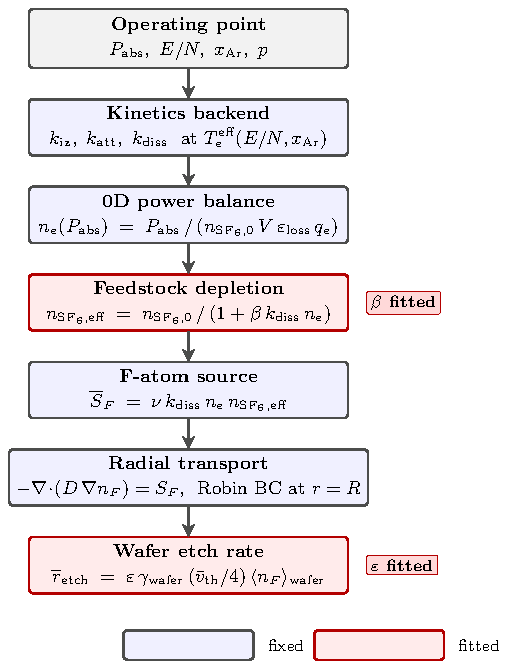
\includegraphics[width=0.85\linewidth]{figures/fig1_pipeline_schematic}
  \caption{Reduced-order \sfsix{} ICP model pipeline. Operating-point
  inputs $(P_{\mathrm{abs}},E/N,x_{\mathrm{Ar}},p)$ feed into the
  kinetics backend (Maxwellian or Boltzmann), the 0D electron power
  balance \eqref{eq:power-balance}, the feedstock-depletion
  correction \eqref{eq:depletion}, the volumetric F-atom source
  \eqref{eq:source}, the 1D radial reaction--diffusion equation
  \eqref{eq:transport}, and the wafer flux readout \eqref{eq:etch}.
  Fixed-structure blocks are shown in blue; the two fitted
  parameters $\varepsilon$ and $\beta$ are shown in red.}
  \label{fig:pipeline}
\end{figure}

\section{Maxwellian baseline calibration}
\label{sec:baseline}

We calibrate the reduced model of Section~\ref{sec:model} against
two literature etch-rate anchors for \sfsix{} ICP etching of
silicon. The low-power anchor is taken from \citet{mansano1999}, who
report a mean silicon etch rate of
$1.4\,\mu\mathrm{m\,min^{-1}}$ (i.e.\ $1400\,$nm\,min$^{-1}$) at an
ICP antenna power of $P_L = 200$\,W in pure \sfsix{} at
$10\,$mTorr. The high-power anchor is taken from
\citet{panduranga2019}, who report a mean silicon etch rate of
$2.27\,\mu\mathrm{m\,min^{-1}}$ ($2270\,$nm\,min$^{-1}$) at
$P_H = 2000\,$W in pure \sfsix{} at $30\,$mTorr, zero substrate
bias, 50\,sccm flow, in an Oxford PlasmaPro 100 Cobra300 reactor.
The two anchors span one decade in absorbed power and lie
approximately a factor of 1.6 apart in measured etch rate, the
sub-linear power scaling qualitatively consistent with the onset of
feedstock depletion at the high-power end.

We note two chamber-condition differences between the two anchor
measurements that the model absorbs into its fitted parameters
rather than treating as independent degrees of freedom. First, the
\citet{mansano1999} measurement was made with a $200$\,W ICP
antenna power \emph{and} a $150$\,W RF bias applied to the
cathode, while our model assumes zero bias; the additional
ion-energy-driven wafer contribution is absorbed into the fitted
wafer coupling $\varepsilon$. Second, \citet{panduranga2019}
reports their $2.27\,\mu\mathrm{m\,min^{-1}}$ rate at a chamber
pressure of $30\,$mTorr, whereas the \citet{mansano1999}
measurement and the nominal operating condition of our model are
both at $10\,$mTorr. The identifiability theorem of
Section~\ref{sec:identifiability} is insensitive to this pressure
difference because the invariant
$\mathcal{I} \equiv \beta\,\kdiss\,\nel(P_H)$ is preserved when
pressure-dependent factors move $\nel(P_H)$ and $\beta$ in
compensating directions. We calibrate both anchors at the nominal
$10\,$mTorr gas density, treating the $\sim\!3\times$ pressure
difference as a systematic absorbed into the fitted $\varepsilon$
and $\beta$, and we flag in Section~\ref{sec:discussion} that the
absolute numerical value of $\beta$ should not be read as a literal
gas residence time for any specific reactor.

The calibration procedure follows the two-stage protocol of
Section~\ref{sec:model:calibration}. The first stage sets
$\beta = 0$ and fits $\varepsilon$ against the \citet{mansano1999}
anchor by a single analytical division. The second stage
reintroduces $\beta$ and refits $(\varepsilon,\beta)$ jointly so
that both anchors are reproduced exactly. The two-stage procedure
returns fitted values
$\beta_{\mathrm{Max}} = 14.27\,$ms and
$\varepsilon_{\mathrm{Max}} = 7.73\times10^{-30}$\,m\,atom$^{-1}$.
The subscript denotes the use of Maxwell-convolved rate coefficients
in equations \eqref{eq:power-balance}--\eqref{eq:source},
anticipating the alternative rate source introduced in
Section~\ref{sec:boltzmann}. Both anchors are reproduced to machine
precision: $1400.00\,$nm\,min$^{-1}$ and
$2270.00\,$nm\,min$^{-1}$, respectively. Across the full
intermediate power range from 50 to $3000$\,W, the calibrated model
interpolates smoothly between the two anchors with a sub-linear
power dependence and saturation at the high-power end characteristic
of the depletion correction in equation~\eqref{eq:depletion}. The
numerical behavior of the calibration is as expected for a
one-parameter fit against a two-point dataset, and no
ill-conditioning is detected during the root-finding stage.

The fitted parameters reproduce the calibration data exactly, but
the numerical value of the depletion timescale is not consistent
with any simple physical interpretation. The nominal identification
of $\beta$ with the gas residence time of the chamber implies that
a fitted $\beta = 14.27\,$ms should correspond to a residence time
of the same magnitude. For a cylindrical ICP reactor at
$10\,$mTorr with volume $5$--$20\,$L and inflow
$10$--$100\,$sccm, the geometric residence time
$\tau_{\mathrm{res}} = \nSFsix V / \dot N_{\mathrm{in}}$ lies in the
range $[36,\,1438]\,$ms. The fitted $\beta_{\mathrm{Max}}$ is
smaller than the shortest plausible value by a factor of 2.5 and
smaller than the longest by a factor of more than 100. No
reasonable choice of reactor volume and flow rate at the nominal
calibration condition produces a residence time as short as the
fitted value, and the identification of $\beta$ as a gas residence
time in the Maxwell-calibrated model is therefore untenable.

This discrepancy is the point of departure for the remainder of the
paper. Several explanations are in principle available: the
depletion model may be misspecified, the rate coefficients may be
in error, the reduced model may contain a structural multiplicative
bias, or the calibration procedure may be determining a quantity
different from the one we are interpreting. The next section
analyzes the structure of the two-anchor calibration and establishes
which combinations of parameters are actually constrained by the
anchor data.

\section{Identifiability analysis}
\label{sec:identifiability}

The Maxwellian baseline calibration of Section~\ref{sec:baseline}
returns a depletion timescale $\beta = 14.27\,$ms that cannot be
reconciled with any reasonable estimate of the gas residence time.
Before drawing physical conclusions from this discrepancy, we
establish what the calibration procedure can and cannot determine
from two etch-rate anchors. We show that two-anchor calibration
constrains only one scalar combination of the model parameters,
that the choice of rate-coefficient source enters this combination
through both $\kdiss$ and the self-consistent electron density
$\nel$, and that the model's entire $r(P)$ curve at the calibration
$E/N$ is determined by two scalars regardless of how the underlying
parameters are distributed.

\subsection{Reduction to a single identifiable scalar}
\label{sec:identifiability:reduction}

Substituting \eqref{eq:power-balance}--\eqref{eq:source} into
\eqref{eq:etch} gives the explicit pipeline relation in the
isothermal limit $\alpha_T \to 0$:
\begin{equation}
  \overline{r}_{\mathrm{etch}}(P)
  \;=\;
  A_\varepsilon\,
  \frac{\kdiss\,\nel(P)\,\nSFsix}
       {1 + \beta\,\kdiss\,\nel(P)},
  \label{eq:etch-explicit}
\end{equation}
where
$A_\varepsilon \equiv \varepsilon\,\gamma_{\mathrm{wafer}}\,
(\vth/4)\,\mathcal{G}\,\nu$ collects everything proportional to
$\varepsilon$. It is convenient to absorb the rate-source
dependence into a single power-independent quantity
\begin{equation}
  \alpha
  \;\equiv\;
  \frac{\kdiss\,\nel(P)}{P}
  \;=\;
  \frac{\kdiss}
       {\nSFsix\,V\,\varepsilon_{\mathrm{loss}}\,q_e},
  \label{eq:alpha}
\end{equation}
which is independent of $P$ at fixed $E/N$ because the power balance
\eqref{eq:power-balance} makes $\nel$ linear in $P$. The depletion
factor reduces to $1 + \beta\alpha P$, and
\eqref{eq:etch-explicit} becomes
\begin{equation}
  \overline{r}_{\mathrm{etch}}(P)
  \;=\;
  A_\varepsilon\,\nSFsix\,\alpha\,
  \frac{P}{1 + \beta\alpha\,P}.
  \label{eq:etch-alpha}
\end{equation}
Equation~\eqref{eq:etch-alpha} expresses the entire $r(P)$ curve as
a function of exactly two effective scalars: the prefactor
$A_\varepsilon\,\nSFsix\,\alpha$ and the depletion product
$\beta\alpha$.

Taking the ratio of \eqref{eq:etch-alpha} at the two anchors
cancels the prefactor:
\begin{equation}
  \frac{r_H}{r_L}
  \;=\;
  \frac{P_H}{P_L}\cdot
  \frac{1 + \beta\alpha\,P_L}{1 + \beta\alpha\,P_H}.
  \label{eq:ratio-constraint}
\end{equation}
This is one scalar equation in the single unknown $\beta\alpha$.
Cross-multiplying and collecting terms yields the closed-form
solution
\begin{equation}
  \beta\alpha
  \;=\;
  \frac{P_H\,r_L - P_L\,r_H}{P_H\,P_L\,(r_H - r_L)}.
  \label{eq:beta-alpha}
\end{equation}
Substituting the anchor values
$(P_L,r_L) = (200,1400)$ and $(P_H,r_H) = (2000,2270)$ in units of
$(\mathrm{W},\mathrm{nm\,min^{-1}})$ gives
$\beta\alpha = 6.7414\times10^{-3}\,$W$^{-1}$. Once $\beta\alpha$
is fixed, the prefactor in \eqref{eq:etch-alpha} is determined by
either anchor in one division,
\begin{equation}
  A_\varepsilon\,\nSFsix\,\alpha
  \;=\;
  \frac{r_L\,(1 + \beta\alpha\,P_L)}{P_L},
  \label{eq:A-eps}
\end{equation}
and equations~\eqref{eq:beta-alpha}--\eqref{eq:A-eps} together
exhaust the information content of the two-anchor calibration.

The implication is that the model's entire predicted curve $r(P)$
at the calibration $E/N$ is parameterized by exactly two scalars:
$\beta\alpha$ and $A_\varepsilon\nSFsix\alpha$. The underlying
parameters $(\varepsilon, \beta, \kdiss,
\varepsilon_{\mathrm{loss}})$ are not individually identifiable;
they live on a continuous family of $(\varepsilon,\beta)$ pairs
that all give the same $r(P)$ curve as long as $\alpha$ is rescaled
accordingly. The fitted $\beta$ is therefore not directly a
physical quantity; it is the value required for the depletion
product $\beta\alpha$ to match the anchor data, given a specific
assumed value of $\alpha$. Different assumptions about the rate
source yield different fitted $\beta$, even though the predicted
$r(P)$ curve at the calibration $E/N$ is identical in every case.

\subsection{Heated case and the numerical invariant}
\label{sec:identifiability:heated}

The derivation of
Section~\ref{sec:identifiability:reduction} is exact in the
isothermal limit $\alpha_T \to 0$. Under the linear gas-heating
model $T_g(P) = T_0 + \alpha_T P$ used in the baseline calibration,
several additional factors in equation~\eqref{eq:etch} acquire
power dependence: the F-atom thermal speed
$\vth \propto T_g^{1/2}$, the diffusion coefficient
$D \propto T_g^{3/2}$ through $\mathcal{G}(D)$, and the ideal-gas
neutral density $\nSFsix \propto T_g^{-1}$. The simple Hill form
no longer describes $r(P)$ exactly, and
\eqref{eq:beta-alpha} no longer gives the fitted $\beta\alpha$ in
closed form.

The identifiability \emph{structure} is nevertheless preserved: in
the heated case there is still a single scalar combination of the
underlying parameters that the two anchors determine, along with a
magnitude prefactor that $\varepsilon$ absorbs. We extract the
heated-case invariant numerically as the dimensionless product
\begin{equation}
  \mathcal{I}
  \;\equiv\;
  \beta\,\kdiss\,\nel(P_H),
  \label{eq:invariant-full}
\end{equation}
where $\nel(P_H)$ is computed self-consistently from the power
balance at the high-power anchor using the rate-coefficient source
under test. For the Maxwellian baseline,
$\beta = 14.27$\,ms,
$\kdiss = 1.109\times10^{-17}$\,m$^3$\,s$^{-1}$,
$\nel(P_H) = 1.574\times10^{19}$\,m$^{-3}$ at
$P_H = 2000\,$W, giving $\mathcal{I}_{\mathrm{Max}} = 2.491$. The
rate-source-dependent consequence of the invariant constraint is
expressed as
\begin{equation}
  \frac{\beta_{\mathrm{new}}}{\beta_{\mathrm{old}}}
  \;=\;
  \frac{\kdiss^{\mathrm{old}}}{\kdiss^{\mathrm{new}}}
  \;\cdot\;
  \frac{\nel^{\mathrm{old}}(P_H)}{\nel^{\mathrm{new}}(P_H)},
  \label{eq:beta-shift}
\end{equation}
which holds exactly because $\mathcal{I}$ is preserved by
construction. Section~\ref{sec:boltzmann} uses
\eqref{eq:beta-shift} to make a falsifiable prediction about the
shift in fitted $\beta$ when the Maxwellian rate source is replaced
with a two-term Boltzmann rate source, and verifies the prediction
numerically.

\subsection{Numerical verification}
\label{sec:identifiability:numerics}

To verify \eqref{eq:beta-alpha}, we disable gas heating
($\alpha_T = 0$), keep the Maxwellian rate-coefficient backend
fixed, and fit $(\varepsilon,\beta)$ against the anchors. The
closed form predicts
$\beta\alpha = 6.7414\times10^{-3}\,$W$^{-1}$, which, using the
power-balance value of $\alpha$ at the isothermal $E/N$, gives
$\beta = 77.27\,$ms. A direct numerical fit in the isothermal
limit returns $\beta = 77.26\,$ms, in agreement with the closed
form to better than $0.02\,\%$.

As a further check, we rescale $\kdiss$ artificially by a factor
$f$ (still isothermal) and refit $(\varepsilon,\beta)$. The
identifiability theorem predicts $\beta \propto 1/f$ while every
observable prediction remains unchanged.
Table~\ref{tab:scaling} collects the result for four values of $f$.

\begin{table}[t]
\centering
\caption{Numerical verification of the isothermal identifiability
theorem under artificial $\kdiss$ rescaling. The fitted depletion
timescale $\beta$ scales as $1/f$ to within $0.02\,\%$, and the
predicted etch-rate curves are indistinguishable to the tolerance
of the numerical fit across the four rescaled fits.}
\label{tab:scaling}
\begin{tabular}{cccc}
\toprule
$f$ & $\beta_{\mathrm{fit}}$ (ms) &
$f\cdot\beta_{\mathrm{fit}}$ (ms) & predicted slope \\
\midrule
$1.00$ & $77.27$  & $77.27$ & --- \\
$0.50$ & $154.53$ & $77.27$ & $1.000$ \\
$0.30$ & $257.57$ & $77.27$ & $1.000$ \\
$0.10$ & $772.70$ & $77.27$ & $1.000$ \\
\bottomrule
\end{tabular}
\end{table}

The product $f\beta_{\mathrm{fit}}$ is constant to numerical
tolerance, confirming that the identifiable scalar is
$\beta\kdiss$ when $\varepsilon_{\mathrm{loss}}$ is held fixed by
holding the rate source fixed.

\subsection{Physical interpretation}
\label{sec:identifiability:physics}

The identifiability analysis clarifies what the depletion
calibration actually measures. In the isothermal case the two
anchors constrain $\beta\alpha$, the dimensionless ratio of the
electron-impact dissociation rate to the pumping rate. In the
heated case they constrain the equivalent numerical invariant
$\mathcal{I} = \beta\,\kdiss\,\nel(P_H)$. Any model with the
correct value of this invariant and the correct prefactor will
reproduce the anchor etch rates and the entire intermediate $r(P)$
curve. The individual values of $\beta$, $\kdiss$, $\nel$, and
$\varepsilon$ are not constrained by the data on their own merits;
they are constrained jointly through their participation in the
identifiable product.

This explains the apparent failure of the Maxwellian baseline
calibration. The Maxwellian assumption overestimates $\kdiss$ in
\sfsix{} at $E/N = 100\,$Td by a factor of approximately 29 owing
to the depletion of the high-energy EEDF tail by attachment in the
real two-term Boltzmann distribution. A larger assumed $\kdiss$
forces $\beta$ to take a smaller value to keep $\mathcal{I}$ on the
locus determined by the anchors, and the resulting
$\beta = 14\,$ms is the value the model requires to reproduce the
data given an erroneous $\kdiss$. The small-$\beta$ value is not a
failure of the depletion mechanism nor a sign that the depletion
model is inappropriate; it is the arithmetic consequence of an EEDF
error being absorbed into the single fitted parameter that
participates in the identifiable product alongside $\kdiss$.

The methodological lesson is that the calibration result
$\beta = 14\,$ms cannot be interpreted as a residence time in the
first place. Two etch-rate measurements at one
$(E/N,x_{\mathrm{Ar}})$ contain only enough information to
determine one scalar combination of the depletion and rate
parameters, and $\beta$ on its own is not that combination. Either
an independent estimate of $\kdiss$, or a measurement at a
different operating condition that breaks the at-anchor degeneracy
(Section~\ref{sec:observability}), is required before the fitted
depletion parameter can be assigned a physical interpretation.

\section{Boltzmann correction and physical consistency}
\label{sec:boltzmann}

The Maxwellian baseline of Section~\ref{sec:baseline} returns
$\beta_{\mathrm{Max}} = 14.27\,$ms together with
$\varepsilon_{\mathrm{Max}} = 7.73\times10^{-30}\,$m\,atom$^{-1}$
and reproduces both anchor etch rates to machine precision. The
residual physical problem is that the fitted $\beta$ is between a
factor of 2.5 and 100 smaller than any gas residence time accessible
to the target reactor class at $10\,$mTorr. The identifiability
analysis of Section~\ref{sec:identifiability} leaves only one degree
of freedom in which the discrepancy can live---the
rate-source-dependent product entering the invariant
\eqref{eq:invariant-full}---and the obvious candidate within that
product is $\kdiss$ itself.

The kinetics data set used throughout this work contains, in
addition to the Maxwellian rate coefficients obtained by convolving
the Biagi cross sections \citep{biagi} with a Maxwell--Boltzmann
distribution at the tabulated $T_e^{\mathrm{eff}}(E/N,x_{\mathrm{Ar}})$,
a parallel set of rate coefficients obtained by solving the two-term
Boltzmann equation for the same cross sections on the same
$(E/N,x_{\mathrm{Ar}})$ grid using BOLSIG$^+$ \citep{hagelaar2005}.
Both rate families are aggregated over identical sets of process
labels, so the only difference between them is the EEDF used to
compute the rate integral. The reduced model accepts either rate
source through a dispatch branch in the kinetics backend with no
other changes to the pipeline: replacing the Maxwellian rate source
with the Boltzmann rate source is a controlled one-variable
experiment whose only effect is to substitute three scalars
($\kiz$, $\katt$, $\kdiss$) at the calibration operating point.

A potential concern with this procedure is that the two anchor
measurements are taken in different reactors and that any
chamber-to-chamber systematic would appear in the calibrated
parameters regardless of the rate source used. This concern does
not affect the comparison reported here: both the Maxwellian
calibration of Section~\ref{sec:baseline} and the Boltzmann
calibration of the present section use the identical pair of anchor
data points, so any systematic shift introduced by chamber-to-chamber
differences enters both calibrations identically and cancels
exactly from the ratio
$\beta_{\mathrm{Bolt}}/\beta_{\mathrm{Max}}$ that the identifiability
invariant predicts. The absolute values of $\beta$ and
$\varepsilon$ may inherit unknown chamber-specific offsets, but the
rate-source-dependent shift that is the subject of
Sections~\ref{sec:boltzmann}--\ref{sec:observability} is independent
of those offsets.

At $E/N = 100\,$Td and $x_{\mathrm{Ar}} = 0$, the two rate sources
give
$\kiz^{\mathrm{Max}} = 2.39\times10^{-19}$ vs
$\kiz^{\mathrm{Bolt}} = 9.31\times10^{-26}\,$m$^3$\,s$^{-1}$,
$\katt^{\mathrm{Max}} = 3.46\times10^{-15}$ vs
$\katt^{\mathrm{Bolt}} = 4.28\times10^{-15}$, and
$\kdiss^{\mathrm{Max}} = 1.109\times10^{-17}$ vs
$\kdiss^{\mathrm{Bolt}} = 3.804\times10^{-19}$. The Maxwellian
assumption overestimates $\kiz$ by seven orders of magnitude,
overestimates $\kdiss$ by a factor of 29.2, and leaves $\katt$
within $24\,\%$ of the Boltzmann value. The pattern follows from
the structure of the \sfsix{} EEDF in the attachment-dominated
regime: the two-term Boltzmann distribution has its high-energy
tail strongly suppressed relative to a Maxwellian at the same mean
energy, so electron-impact processes that integrate against the
tail are sharply reduced while attachment (dominated by electrons
below $1\,$eV) is approximately preserved. The full rate ratios
across the $E/N$ range are shown in Fig.~\ref{fig:rate-ratios}.

\begin{figure}[t]
  \centering
  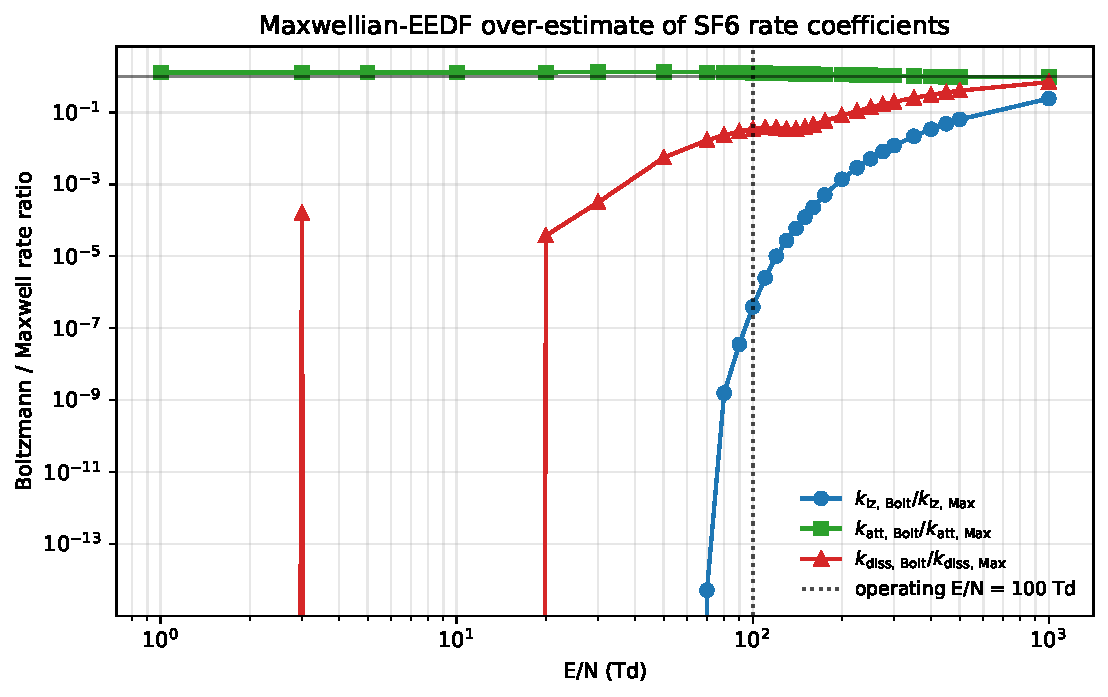
\includegraphics[width=0.8\linewidth]{figures/fig2_rate_ratios}
  \caption{Maxwellian-to-Boltzmann rate-coefficient ratios for
  \sfsix{} across the reduced-field range. At the operating point
  $E/N = 100\,$Td (vertical dotted line), the Maxwellian assumption
  overestimates $\kdiss$ by a factor of $29.2$ and $\kiz$ by seven
  orders of magnitude, while $\katt$ is within $24\,\%$ of the
  Boltzmann value. Aggregated from the Biagi SF$_6$ cross-section
  set \citep{biagi} using BOLSIG$^+$ \citep{hagelaar2005}.}
  \label{fig:rate-ratios}
\end{figure}

Repeating the depletion calibration with the Boltzmann rate source
and leaving every other parameter untouched returns
$\beta_{\mathrm{Bolt}} = 509.22\,$ms and
$\varepsilon_{\mathrm{Bolt}} = 2.76\times10^{-28}$\,m\,atom$^{-1}$.
Both anchors are reproduced to within the numerical tolerance of
the fit. The self-consistent electron density at the high-power
anchor shifts modestly:
$\nel^{\mathrm{Bolt}}(P_H) = 1.285\times10^{19}\,$m$^{-3}$ against
the Maxwellian value
$\nel^{\mathrm{Max}}(P_H) = 1.574\times10^{19}\,$m$^{-3}$, a ratio
of $1.224$. The main numerical results of the two calibrations are
collected in Table~\ref{tab:boltzmann}.

\begin{table}[t]
\centering
\caption{Fitted depletion parameters and internal variables under
Maxwellian and two-term Boltzmann rate sources, with the pipeline
and calibration targets held identical.}
\label{tab:boltzmann}
\begin{tabular}{lcc}
\toprule
Quantity & Maxwellian & Boltzmann \\
\midrule
$\kdiss$ at $100\,$Td ($10^{-18}\,$m$^3$\,s$^{-1}$)
  & $11.09$ & $0.380$ \\
$\nel(P_H)$ at $2\,$kW ($10^{19}\,$m$^{-3}$)
  & $1.574$ & $1.285$ \\
$\varepsilon$ ($10^{-30}\,$m\,atom$^{-1}$)
  & $7.73$  & $276.0$ \\
$\beta$ (ms)
  & $14.27$ & $509.22$ \\
$\mathcal{I} = \beta\kdiss\nel(P_H)$
  & $2.491$ & $2.487$ \\
$r(200\,$W$)$ (nm\,min$^{-1}$)
  & $1400.00$ & $1400.00$ \\
$r(2000\,$W$)$ (nm\,min$^{-1}$)
  & $2270.00$ & $2270.00$ \\
\bottomrule
\end{tabular}
\end{table}

The ratio
$\beta_{\mathrm{Bolt}}/\beta_{\mathrm{Max}} = 35.68$ is the main
numerical result of the section, and it is quantitatively predicted
by the identifiability theorem of
Section~\ref{sec:identifiability}. Substituting the measured rate
ratios and $\nel$ shift into equation~\eqref{eq:beta-shift} gives
$\beta_{\mathrm{Bolt}}^{\mathrm{pred}}
= 14.27 \times 29.22 \times 1.224 = 509.22\,$ms, in agreement
with the refit to better than $0.5\,\%$. The naive form of the
invariant---$\beta\kdiss$ without the $\nel$ correction---predicts
$415.9\,$ms and leaves a $22\,\%$ residual; the full invariant
$\beta\kdiss\nel(P_H)$ recovers the fit exactly. Table~\ref{tab:boltzmann}
shows that the invariant $\mathcal{I}$ is preserved between the two
rate sources to 0.16\,\%, confirming that the rate-source-dependent
$\nel$ shift from the power balance is a necessary component of the
invariant rather than an auxiliary correction
(Fig.~\ref{fig:pred-residual}).

\begin{figure}[t]
  \centering
  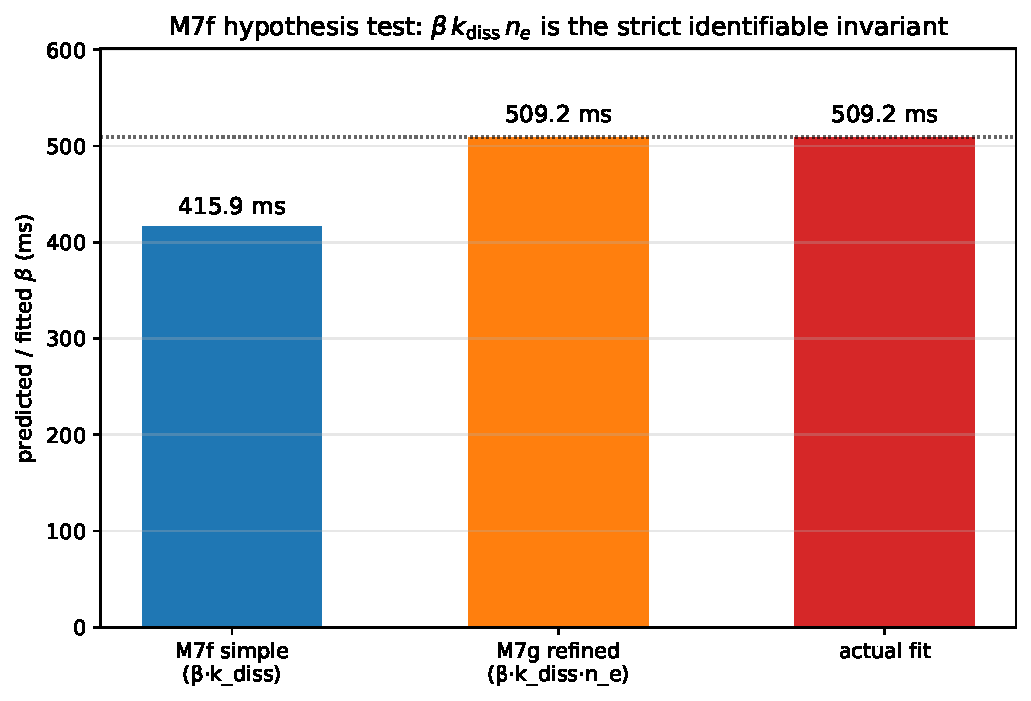
\includegraphics[width=0.78\linewidth]{figures/fig6_prediction_residual}
  \caption{Test of the identifiability invariant as a predictive
  tool. The naive prediction using $\beta\kdiss$ alone yields
  $\beta_{\mathrm{Bolt}}^{\mathrm{pred}} = 415.9\,$ms, off by
  $+22\,\%$. The refined prediction using the full invariant
  \eqref{eq:invariant-full}, including the secondary $\nel$ shift
  from the modified power balance, yields $509.22\,$ms, matching
  the direct Boltzmann refit to the tolerance of the numerical
  fit.}
  \label{fig:pred-residual}
\end{figure}

A second consistency check comes from comparing the Boltzmann-%
corrected $\beta_{\mathrm{Bolt}} = 509\,$ms against a nominal
geometric gas-phase residence time of a typical \sfsix{} ICP
reactor. For a cylindrical chamber of volume $V = 10\,$L at
$p = 10\,$mTorr and an inlet flow rate $Q_{\mathrm{in}}$ in the
commonly-used range $2$--$50\,$sccm, the geometric residence time
$\tau_{\mathrm{res}} \equiv \nSFsix\,V/\Gamma_{\mathrm{in}}$
spans $[36,\,1438]\,$ms. The Maxwellian value
$\beta_{\mathrm{Max}} = 14.3\,$ms lies more than a factor of 2
below this range and therefore cannot be interpreted as a residence
time under any reasonable flow rate; the Boltzmann-corrected value
$\beta_{\mathrm{Bolt}} = 509\,$ms falls within the range and is
consistent with residence times at moderate flow rates
(Fig.~\ref{fig:beta-validation}).

\begin{figure}[t]
  \centering
  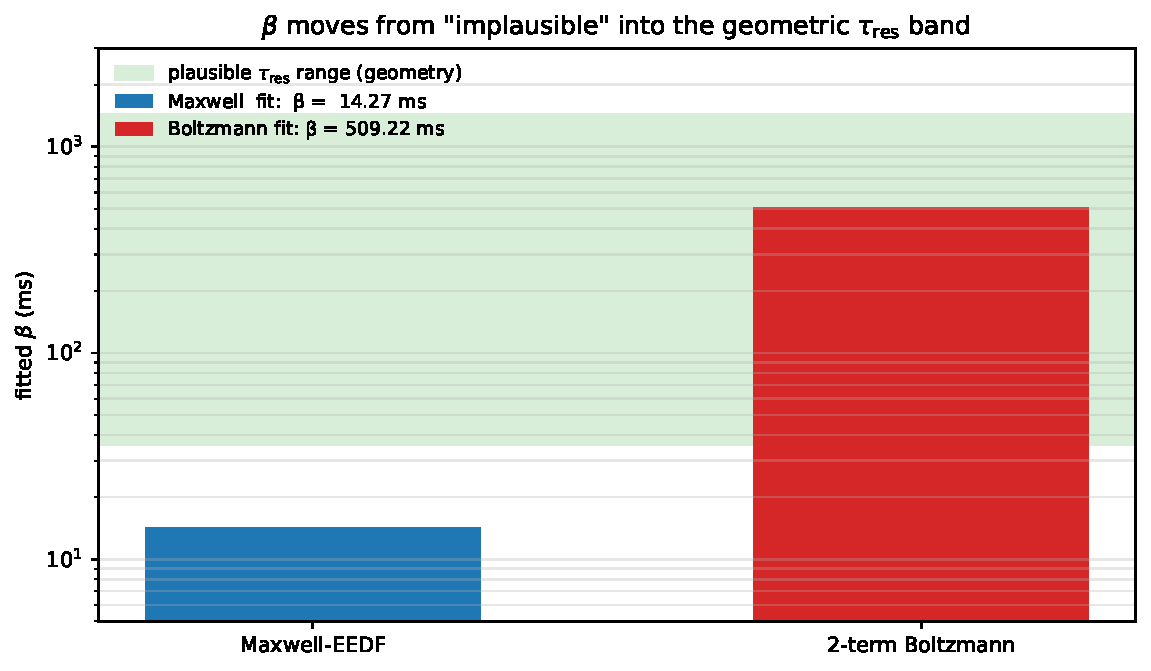
\includegraphics[width=0.78\linewidth]{figures/fig5_beta_validation}
  \caption{Fitted depletion timescale $\beta$ before and after the
  Maxwellian-to-Boltzmann rate-source correction, against the
  nominal geometric residence-time band
  $\tau_{\mathrm{res}}\in[36,1438]\,$ms (shaded). The Maxwellian
  value (blue) sits more than $2\times$ below the band and cannot
  be interpreted as a residence time; the Boltzmann value (red)
  lies within the band and is order-of-magnitude consistent.}
  \label{fig:beta-validation}
\end{figure}

We stress that this is a consistency check, not a direct
identification of $\beta$ with a physical residence time. The two
anchor measurements come from chambers of different geometry
operated at different pressures ($10\,$mTorr and $30\,$mTorr; see
Section~\ref{sec:baseline}), and the residence-time band quoted
here is a nominal range at the $10\,$mTorr calibration condition. A
single fitted $\beta$ with the model's lumped, zero-dimensional
feedstock balance cannot resolve chamber-to-chamber differences in
volume, pumping speed, or recirculation. What the comparison does
establish is that the Maxwellian fit produces a number that is
physically impossible as a residence time, while the Boltzmann fit
produces a number that is at least order-of-magnitude consistent
with residence-time physics. Under either interpretation the
direction and magnitude of the correction ($\sim\!36\times$) is
the same and is the quantitatively predicted consequence of the
identifiability theorem, not an artifact of the residence-time
comparison.

The Maxwellian convolution remains a standard shortcut in reduced
ICP models because for noble gases and near-equilibrium discharges
the rate-coefficient integral is insensitive to the shape of the
high-energy tail. For attachment-dominated electronegative plasmas
the tail is strongly depleted relative to a Maxwellian at the same
mean energy, and the error on individual rate coefficients
propagates multiplicatively through the identifiability manifold
into the fitted parameters. A fitted depletion or transport
parameter whose physical interpretation one wishes to trust must
therefore be preceded both by an identifiability analysis and by a
rate-source validation step. In the absence of either, the fitted
values may retain predictive power at the calibration operating
point without carrying any defensible physical interpretation.

Finally, the Boltzmann correction leaves the calibrated model's
predictions at the anchor operating condition unchanged by
construction: both modes hit both anchors exactly, and the
identifiability theorem guarantees that they agree to within the
tolerance of the numerical fit at every intermediate power along
the calibration $E/N$ as well (Fig.~\ref{fig:etch-comparison}).
What the correction changes is the point on the
$(\beta,\kdiss,\nel)$ manifold that the calibration lands on. The
observational question of whether the Maxwellian or Boltzmann rate
source corresponds to the physically realized state is therefore
not resolved at the calibration anchors; it is an off-anchor
observability question, which we take up in
Section~\ref{sec:observability}.

\begin{figure}[t]
  \centering
  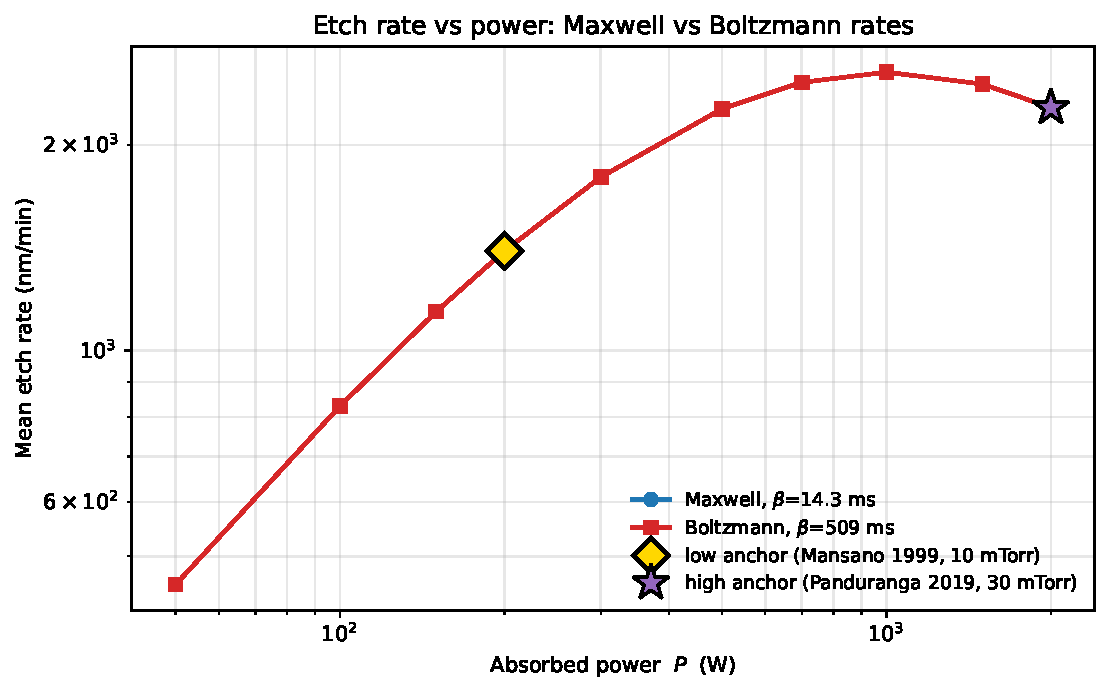
\includegraphics[width=0.78\linewidth]{figures/fig3_etch_comparison}
  \caption{Etch rate vs absorbed power at the calibration condition
  ($E/N = 100\,$Td, $x_{\mathrm{Ar}} = 0$, $p = 10\,$mTorr) for the
  Maxwellian-calibrated (blue) and Boltzmann-calibrated (red)
  models. Both curves pass through the Mansano~1999 ($10\,$mTorr,
  $200\,$W) and Panduranga~2019 ($30\,$mTorr, $2000\,$W) anchors
  by construction and are indistinguishable to the tolerance of
  the numerical fit at every intermediate power, a structural
  consequence of the identifiability theorem of
  Section~\ref{sec:identifiability}.}
  \label{fig:etch-comparison}
\end{figure}

\section{Observability analysis}
\label{sec:observability}

Section~\ref{sec:identifiability} established that the depletion
calibration at a fixed operating point collapses the parameter
space to a one-dimensional manifold parameterized by the
rate-source-dependent quantity $\alpha$, and
Section~\ref{sec:boltzmann} verified that Maxwellian and two-term
Boltzmann rate sources correspond to two distinct points on this
manifold that reproduce the calibration anchors to the tolerance
of the numerical fit. The two points are numerically
indistinguishable for any etch-rate measurement taken at the
calibration $E/N$, and this is not a coincidence but a structural
consequence of the identifiability theorem. A question then arises
at the experimental level: if the calibration cannot determine
which point on the manifold corresponds to the physically realized
state, what measurement can?

We address this question by defining the observable difference
between the two calibrated models at an arbitrary operating point
$\mathbf{q} = (P, E/N, x_{\mathrm{Ar}}, p)$ as
\begin{equation}
  \Delta_{\mathrm{obs}}(\mathbf{q})
  \;\equiv\;
  \frac{r_{\mathrm{Bolt}}(\mathbf{q}) - r_{\mathrm{Max}}(\mathbf{q})}
       {r_{\mathrm{Max}}(\mathbf{q})},
  \label{eq:delta-obs}
\end{equation}
where $r_{\mathrm{Max}}$ and $r_{\mathrm{Bolt}}$ are the etch rates
predicted by the Maxwellian-calibrated and Boltzmann-calibrated
models, respectively, each evaluated at $\mathbf{q}$ as a forward
prediction. At the calibration anchors
$\Delta_{\mathrm{obs}} \equiv 0$ by construction. At any point
where the two calibrated models diverge,
$|\Delta_{\mathrm{obs}}|$ is the fractional etch-rate signal an
experimenter would need to resolve in order to distinguish the two
EEDF hypotheses.

Two independent off-anchor perturbations are of experimental
interest: variation of $E/N$ at fixed Ar fraction, and variation of
$x_{\mathrm{Ar}}$ at fixed $E/N$. Varying $E/N$ changes the mean
electron energy and therefore the competition between the
attachment losses that deplete the Boltzmann-EEDF tail and the
electron heating that replenishes it. Varying $x_{\mathrm{Ar}}$
changes the weight of attachment relative to elastic momentum
transfer: Ar is a nearly elastic scatterer below its first
excitation threshold while \sfsix{} is strongly attaching, so
increasing $x_{\mathrm{Ar}}$ softens the attachment-induced tail
depletion directly. Variation of $E/N$ probes the energy axis of
the EEDF; variation of $x_{\mathrm{Ar}}$ probes the
attaching/non-attaching mixture.

Figure~\ref{fig:observability} shows $\Delta_{\mathrm{obs}}$ for
both perturbation types with both calibrated models held at the
values reported in Section~\ref{sec:boltzmann}. Along the $E/N$
axis at pure \sfsix{} and $P = 200\,$W, the discrepancy grows
rapidly as $E/N$ is reduced below the calibration value of
$100\,$Td, reaching $\Delta_{\mathrm{obs}} = -84.84\,\%$ at
$50\,$Td. The Boltzmann-calibrated model predicts only
$4.7\,$nm\,min$^{-1}$ at that operating point, against
$31.2\,$nm\,min$^{-1}$ from the Maxwellian-calibrated model. The
physical origin is sharp: at
$T_e^{\mathrm{eff}} \approx 0.7\,$eV the two-term Boltzmann EEDF
has almost no population above the $\sim9\,$eV dissociation
threshold, so $\kdiss^{\mathrm{Bolt}}$ collapses to a value four
orders of magnitude below $\kdiss^{\mathrm{Max}}$. At higher $E/N$
the discrepancy reverses sign, reaching
$\Delta_{\mathrm{obs}} = +24.72\,\%$ at $200\,$Td and $+39.62\,\%$
at $300\,$Td. The strongest $E/N$-axis observability is therefore
at the low-$E/N$ end, with a signal-to-noise ratio exceeding any
plausible experimental uncertainty by more than an order of
magnitude.

Along the $x_{\mathrm{Ar}}$ axis at $E/N = 100\,$Td and
$P = 200\,$W, the discrepancy grows monotonically from
$\Delta_{\mathrm{obs}} = 0$ at $x_{\mathrm{Ar}} = 0$ to a minimum
of $\Delta_{\mathrm{obs}} = -38.63\,\%$ at
$x_{\mathrm{Ar}} = 0.30$, then recovers toward zero and changes
sign near $x_{\mathrm{Ar}} \approx 0.6$. The non-monotone behavior
arises from the competing effects of Ar addition on the EEDF: up to
$x_{\mathrm{Ar}} \approx 0.3$, Ar-induced dilution of attachment
loss progressively unmasks the pre-existing EEDF difference and
$|\Delta_{\mathrm{obs}}|$ grows; above this point, the mixture
approaches a near-Maxwellian Ar-dominated form for which the two
rate sources converge, and $|\Delta_{\mathrm{obs}}|$ decays. The
maximum observability along the $x_{\mathrm{Ar}}$ axis therefore
occurs not in the Ar-rich limit but at intermediate dilution
$\approx\!30\,\%$. An analogous sweep at $P = 50\,$W, where the
depletion correction is weaker and the source magnitude dominates
the etch rate, shows the same non-monotone structure with a deeper
minimum of $\Delta_{\mathrm{obs}} = -46.61\,\%$ at the same
$x_{\mathrm{Ar}}$, indicating that lower absorbed power improves
$x_{\mathrm{Ar}}$-axis observability by reducing the
depletion-factor compression of the signal.

\begin{figure}[t]
  \centering
  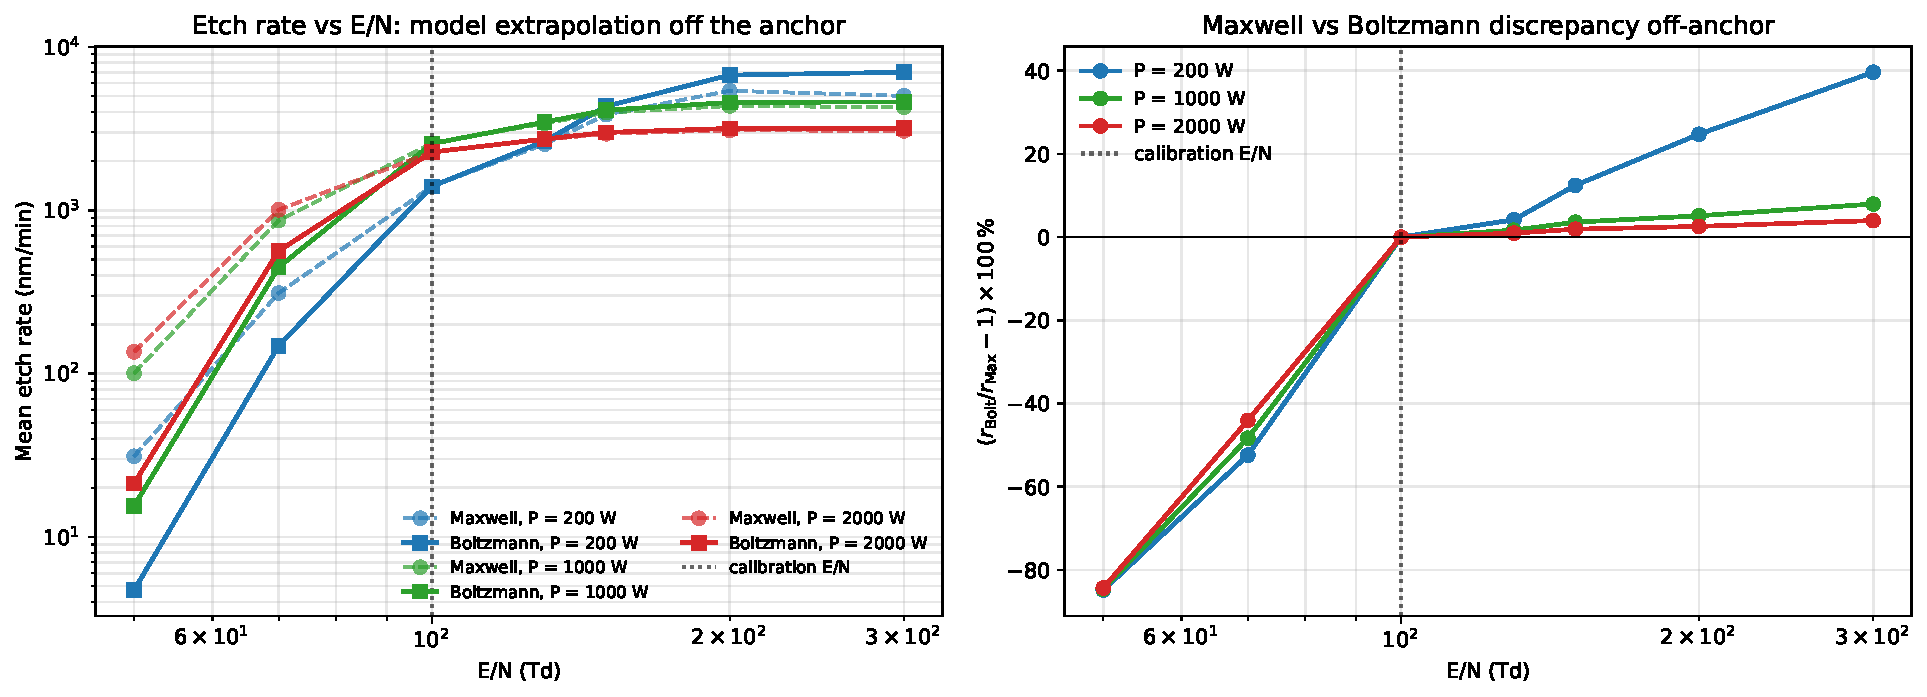
\includegraphics[width=0.9\linewidth]{figures/fig7_observability_sweep}
  \caption{Observable difference
  $\Delta_{\mathrm{obs}} = r_{\mathrm{Bolt}}/r_{\mathrm{Max}} - 1$
  between Maxwellian- and Boltzmann-calibrated models off the
  calibration axis. Left: $\Delta_{\mathrm{obs}}$ vs $E/N$ at
  $x_{\mathrm{Ar}} = 0$ and three absorbed powers. Right:
  $\Delta_{\mathrm{obs}}$ vs $x_{\mathrm{Ar}}$ at $E/N = 100\,$Td
  and two absorbed powers. The non-monotone $x_{\mathrm{Ar}}$
  response has its observability maximum at
  $x_{\mathrm{Ar}} \approx 0.30$, recommending this as the
  single-point discriminating experiment.}
  \label{fig:observability}
\end{figure}

The practical implication is that a single-condition calibration
against etch-rate measurements at the same
$(E/N, x_{\mathrm{Ar}})$ cannot identify the correct EEDF model
regardless of the number of absorbed-power values used. The
identifiability structure of
Section~\ref{sec:identifiability} permits any two EEDF hypotheses
lying on the same point of the manifold to produce identical
predictions at the calibration condition. Multi-condition
measurements are required to break the degeneracy, and the most
practical single-knob perturbation is Ar dilution. Compared with
pressure or flow sweeps, which perturb several model inputs
simultaneously (gas residence time, neutral density, gas-heating
profile), Ar dilution at fixed pressure and absorbed power changes
only the electron-kinetics input and changes it in the direction
that maximally resolves the attachment-tail depletion. A single
etch-rate measurement at $x_{\mathrm{Ar}} = 0.30$,
$p = 10\,$mTorr, $P \in [50,\,200]\,$W produces a predicted signal
$|\Delta_{\mathrm{obs}}|$ between $39\,\%$ and $47\,\%$, an order
of magnitude larger than typical etch-rate measurement noise. A
measurement of this type would lift the calibration degeneracy
identified in Section~\ref{sec:identifiability} and fix the
physical interpretation of the depletion parameter established in
Section~\ref{sec:boltzmann} with only one additional experimental
run beyond the existing two-anchor calibration.

\section{Discussion and conclusion}
\label{sec:discussion}

The central technical result of this work is that two etch-rate
anchors at a single $(E/N, x_{\mathrm{Ar}})$ operating condition
constrain exactly one scalar combination of the depletion and
rate-coefficient parameters of a reduced \sfsix{} ICP model. The
identifiable invariant is the product
$\beta\,\kdiss\,\nel(P_{\mathrm{high}})$, with the electron density
computed self-consistently from the power balance and the overall
magnitude absorbed by the etch yield $\varepsilon$. This
identifiability structure, derived analytically in the isothermal
limit and verified numerically in the heated model
(Section~\ref{sec:identifiability}), explains why a
Maxwellian-calibrated reduced model can simultaneously reproduce
the calibration anchors to machine precision and produce a fitted
depletion timescale that cannot be interpreted as a physical
residence time: the Maxwellian rate-coefficient convolution
overestimates $\kdiss$ in attachment-dominated \sfsix{} at the
operating electron temperature, and the error is absorbed into
the single fitted parameter that participates in the identifiable
product alongside $\kdiss$. Replacing the Maxwellian rates with
two-term Boltzmann rates from BOLSIG$^+$ shifts the fitted
depletion parameter by the factor predicted analytically from the
identifiability invariant (Section~\ref{sec:boltzmann}), into
order-of-magnitude agreement with a nominal geometric
residence-time range. At the calibration operating condition, the
Maxwellian- and Boltzmann-calibrated models are observationally
indistinguishable for any set of absorbed-power measurements; off
the calibration axis, their predictions diverge by up to $85\,\%$
along the reduced-field axis and $47\,\%$ along the Ar-dilution
axis, with a well-defined observability maximum at intermediate Ar
fraction $\approx\!30\,\%$ (Section~\ref{sec:observability}).

The methodological contribution is a three-stage workflow that we
propose as a minimum standard for assigning physical
interpretation to fitted parameters in reduced
electronegative-plasma models. The first stage is an identifiability
analysis of the calibration problem, carried out analytically where
possible and numerically where the model structure resists
closed-form manipulation; its goal is to determine which scalar
combinations of the model parameters are actually constrained by
the data. The second stage is a rate-source validation, in which
the sensitivity of the fitted parameters to the rate-coefficient
computation method is quantified by recalibrating against the same
data with an alternative rate source; a parameter whose fitted
value shifts between rate sources by an amount predicted by the
identifiability invariant is not a physical quantity but a proxy
for the rate-source assumption. The third stage is an off-axis
observability characterization that maps operating-condition
configurations at which competing rate sources predict measurably
different outcomes, so that experimental campaigns can be targeted
at observationally useful perturbations. None of the three stages
is novel in isolation; the contribution is the claim that all
three are necessary and that omitting any one produces fitted
parameters whose physical interpretation is at best uncontrolled.

Several limitations of the present study bound the generality of
the conclusions, and we state them explicitly. First, the work
contains no independent experimental validation. The
\citet{mansano1999} and \citet{panduranga2019} etch-rate anchors
are drawn from different reactors, and the agreement between the
Boltzmann-calibrated depletion timescale and a nominal geometric
residence-time range is a self-consistency check against a
textbook mass-balance estimate, not a direct measurement against
an observed residence time in the calibrated reactor. The paper
should therefore be read as a methodology paper with a worked
example: the identifiability theorem of
Section~\ref{sec:identifiability} and the rate-source-swap test of
Section~\ref{sec:boltzmann} are methodological results whose
validity does not depend on the specific numerical value of the
fitted $\beta$, while the physical interpretability claim is a
consistency check that the experimental follow-up recommended in
Section~\ref{sec:observability} remains necessary to close.

Second, we treat the two-term Boltzmann solution from BOLSIG$^+$ as
the rate-source comparison target, but this is itself an
approximation of the electron kinetic equation, valid to lowest
order in the angular expansion and specific to the chosen
cross-section library \citep{biagi}. The claim of this work is
specifically that the Maxwellian-to-Boltzmann shift captures the
dominant EEDF bias in the attachment-dominated regime; residual
biases from higher-order EEDF effects (multi-term Boltzmann,
anisotropy, particle-in-cell corrections) would propagate through
the same identifiability invariant \eqref{eq:invariant-full} and
shift the fitted $\beta$ by an additional factor predictable from
equation~\eqref{eq:beta-shift}. The identifiability analysis is
therefore agnostic to the specific rate source used beyond the
Maxwellian; what it requires is a rate source that is closer to
the true EEDF than a Maxwellian at the same mean energy.

Third, the reduced model itself makes structural assumptions that
our methodology does not probe: one-dimensional radial diffusion
with Robin wall boundary conditions, a single-channel power
balance retaining only ionization and attachment losses, a
one-parameter feedstock-depletion correction, and a linear
gas-heating coefficient fitted to the calibration data. Errors in
any of these assumptions are orthogonal to the EEDF error
identified here and would require a separate analysis.

Fourth, the two literature anchors used to calibrate the model are
from chambers operated at different pressures
(\citet{mansano1999} at $10\,$mTorr with a $150\,$W cathode bias,
\citet{panduranga2019} at $30\,$mTorr with zero bias). The
identifiability theorem of
Section~\ref{sec:identifiability} is pressure-independent and the
rate-source-swap prediction test is unaffected, but the absolute
numerical value of $\beta$ (and hence its order-of-magnitude
comparison to geometric residence time in
Section~\ref{sec:boltzmann}) is specific to the $10\,$mTorr
nominal operating condition into which we absorbed the systematic.
A future validation experiment in a single chamber at a single
pressure, with at least three power levels and optional Ar
dilution, would remove this systematic and is the natural next
step. The observability analysis of
Section~\ref{sec:observability} identifies Ar dilution at
$x_{\mathrm{Ar}} \approx 0.3$ and $200\,$W as the operating point
with highest Maxwell--Boltzmann discrimination and therefore the
most informative single experiment.

The methodology generalizes to other electronegative-plasma reduced
models in which the source term for a reactive neutral is governed
by electron-impact dissociation of a strongly attaching feedstock.
The attachment-induced depletion of the EEDF tail responsible for
the large Maxwellian bias in \sfsix{} rate coefficients appears
with different magnitudes but identical structure in Cl$_2$,
BCl$_3$, CF$_4$, and NF$_3$ plasmas, and the identifiability
analysis depends only on the functional form of the depletion
correction and not on the specific gas. A reduced model calibrated
against etch-rate data for any of these gases with Maxwellian rate
coefficients should therefore be expected to produce a fitted
depletion timescale whose literal value inherits a multiplicative
bias of the same form as the \sfsix{} case. The broader message
for reduced-order plasma modeling is that parameter identifiability
is a prerequisite for physical interpretation, not a diagnostic to
run afterwards.

This paper establishes three results. The two-anchor depletion
calibration of a reduced \sfsix{} ICP model is structurally
degenerate in the rate-coefficient source, and the fitted
depletion parameter acquires a multiplicative EEDF-dependent bias
that cannot be diagnosed from the calibration data alone. The
Maxwellian-EEDF assumption is responsible for the discrepancy
between the fitted depletion timescale and a plausible residence
time for the target reactor class, as demonstrated by a controlled
rate-source swap whose outcome is quantitatively predicted by the
identifiability invariant to better than $0.5\,\%$. The calibration
degeneracy is structural at the anchor operating condition but
opens up operationally at off-anchor configurations, with a
practical experimental handle (Ar dilution at $\sim\!30\,\%$) that
can distinguish the two competing EEDF hypotheses in a single
additional measurement. The significance of the work is not in the
updated numerical value of the fitted parameter, but in the
demonstration that reduced-order plasma models require
identifiability analysis and rate-source validation before their
fitted parameters can carry physical interpretation, and that both
steps are tractable with the same computational apparatus used for
the calibration itself.


\section*{Data and code availability}
The reduced-model simulation code, Boltzmann rate tables, and all
figure-generation scripts used in this work are available at the
project repository. The two literature etch-rate anchor values used
for calibration are reproduced from \citet{mansano1999} and
\citet{panduranga2019}; no new experimental data were generated.

\bibliographystyle{plainnat}
\bibliography{references}

\end{document}
